\begin{savequote}[75mm]
Strike hot iron and call forth sparks; strike a man and call forth fury; to shape man or metal to thy will, thou must
strike with force.
\qauthor{Collected Sermons of Carras, Thief by Looking Glass Studios}
\end{savequote}

\chapter{Eksperyment numeryczny}
\newthought{Lorem ipsum dolor sit amet}, consectetuer adipiscing elit. Morbi commodo, ipsum sed pharetra gravida, orci
\section{Metodyka}
We conduct numerical simulations with the aid of a parallel MHD code PIERNIK
using the cylindrical coordinate system. 
Following \cite{M07} and \cite{SO10} we use ''angular momentum-conserving form''
of the $\phi$-momentum equation, which with respect to Cartesian geometry
introduces only one additional source term to equations~\mref{eq3} - \mref{eq4}:
$\left((\rho_g u_\phi + P) / R\right)\mathbf{\hat{R}}$ and $(\rho_d w_\phi / R)
\mathbf{\hat{R}}$ respectively.


\subsection{Podstawowe równania}
Globalna dynamika dysku okołogwiazdowego opisujemy poprzez dwa, wzajemnie ze
sobą oddziałujące płyny: neutralny gaz podlegający izotermicznemu równaniu
stanu oraz pył jako bezciśnieniowy płyn. Równania hydrodynamiki przyjmują dla
takiego modelu następującą postać:

% CONSERVATIVE FORM
\begin{align}
\partial_t \rho_g &+ \nabla\cdot\left(\rho_g\mathbf{u}\right) = 0,\\
\partial_t \rho_d &+ \nabla\cdot\left(\rho_d\mathbf{w}\right) = 0,\\
\partial_t \left(\rho_g\mathbf{u}\right) &+
   \nabla\cdot(\mathbf{u}\otimes(\rho_g\mathbf{u})+P) \notag\\
 &= -\rho_g\left(\nabla\Phi +
\frac{\rho_d}{\tau_f\rho_g}(\mathbf{u}-\mathbf{w})\right),\label{eq3}\\
\partial_t \left(\rho_d\mathbf{w}\right) &+
\nabla\cdot(\mathbf{w}\otimes(\rho_d\mathbf{w})) \notag\\
 &= -\rho_d\left(\nabla\Phi + \frac{1}{\tau_f}(\mathbf{w}-\mathbf{u})\right)
\label{eq4}.
\end{align}
% NON-CONSERVATIVE FORM
%\begin{align}
%\partial_t \rho_g &+ \nabla\cdot\left(\rho_g\mathbf{u}\right) = 0,\\
%\partial_t \rho_d &+ \nabla\cdot\left(\rho_d\mathbf{w}\right) = 0,\\
%\partial_t \mathbf{u} &+ \left(\mathbf{u}\cdot\nabla\right)\mathbf{u} = 
% -\nabla\Phi + \frac{\rho_d}{\tau_f\rho_g}(\mathbf{w}-\mathbf{u})
% -c_s^2\nabla\ln\rho_g,\label{eq3} \\
%\partial_t \mathbf{w} &+ \left(\mathbf{w}\cdot\nabla\right)\mathbf{w} = 
% -\nabla\Phi - \frac{1}{\tau_f}(\mathbf{w}-\mathbf{u}),\label{eq4}
%\end{align}

\noindent gdzie $\rho_g$, $\rho_d$ to odpowiednio gęstości gazu i pyłu,
$\mathbf{u}$, $\mathbf{w}$ ich prędkości, $P$ to ciśnienie gazu, $\tau_f$ jest
skalą czasową tarcia~\footnote{ang. friction time}, a $\Phi$ to potencjał
grawitacyjny. Naszym celem jest wyizolowanie niestabilności strumieniowej z
pośród szeregu innych procesów, które mogą zachodzić w powyższym modelu. Z tego
względu zaniedbujemy pionową składową przyspieszenia grawitacyjnego pochodzącą
od centralnego obiektu w dysku, która prowadziła by do naturalnej sedymentacji
pyłu w płaszczyźnie dysku i wzbudzenia się niestabilności
Kelvina-Helmholtza~\cite{JHK06}.

W ramach pracy skupiono się na dyskach rozciągających się relatywnie dużych
promienii tj. 2~AU. Zakładając, za pracą~\cite{CD93}, że przejście do
reżimu Stokesa zachodzi dla ziaren pyłu o promieniu większym niż
$a = 9/4\lambda_g$ gdzie $\lambda_g = 4.2\times 10^4\textrm{
cm} (10^{-14}\textrm{ g cm}^{-3}/\rho_g) \approx (R/1 \textrm{AU})^{2.75}$~cm 
jest średnią drogą swobodną molekuł gazu~\citep{W77,BT09}, zaś $R$ jest
odległością radialną od centrum dysku. Przy tych założeniach, reżim Epstein ma
zastosowanie dla dominującej części domeny obliczeniowej nawet dla największych
symulowanych przez nas ziaren pyłu. Skala czasowa tarcia przyjmuję zatem
następującą postać:
%
\begin{equation}
   \tau_f = \frac{\rho_\bullet a} 
      {\rho_g \sqrt{c_s^2 + |\mathbf{u} - \mathbf{w}|^2 }}
   \label{eq:tauf} 
\end{equation}
%
gdzie $c_s$ jest prędkością dźwięku w gazie, zaś $\rho_\bullet = 1.6\textrm{ g cm}^{-3}$
jest gęstością materiału z którego zbudowany jest pył. Po mimo faktu, że wyraz
$|\mathbf{u}-\mathbf{w}|^2$ nie odgrywa znaczącej roli podczas ewolucji
niestabilności strumieniowej, t.j. jego wartość nie przekracza nigdy 1 procenta
prędkości dźwięku, postanowiliśmy go nie zaniedbywać ze względu na
kompletność {\bf blah}
%
\begin{figure*}
   \centering
   \begin{tabular}{@{}cc@{}}
      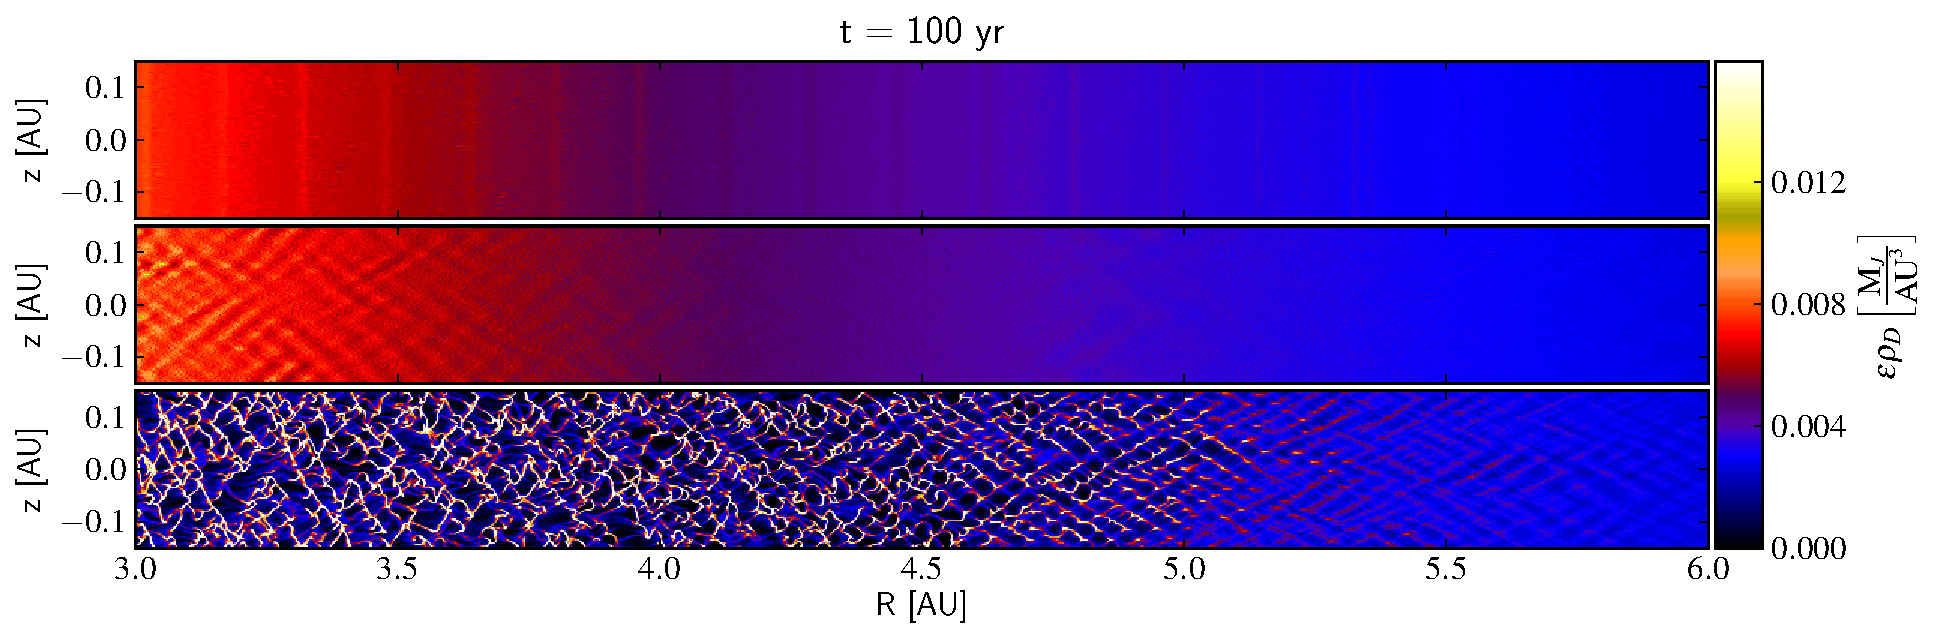
\includegraphics[width=0.49\linewidth]{figures/fig1a} & 
      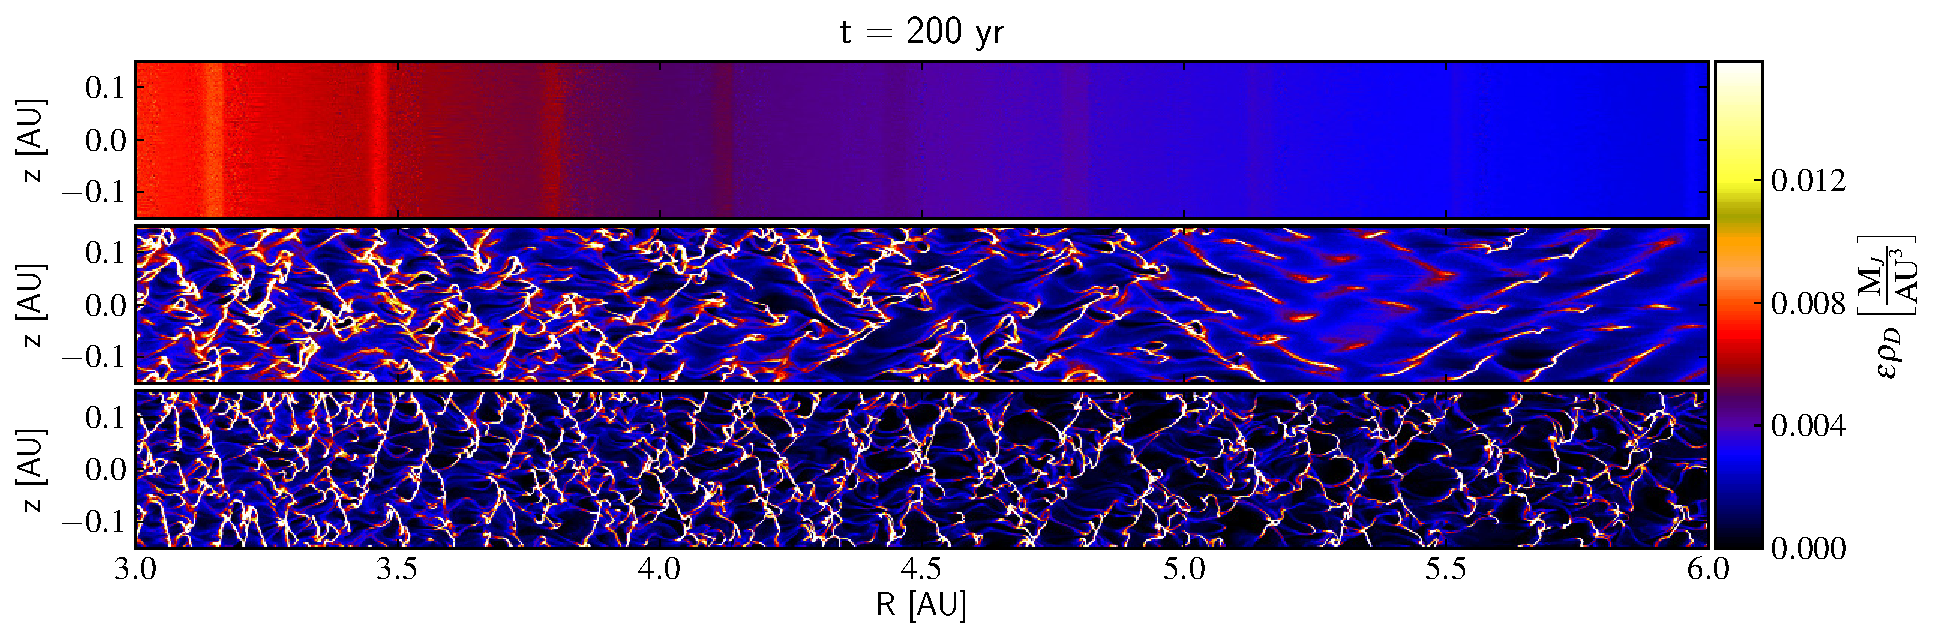
\includegraphics[width=0.49\linewidth]{figures/fig1b} \\
      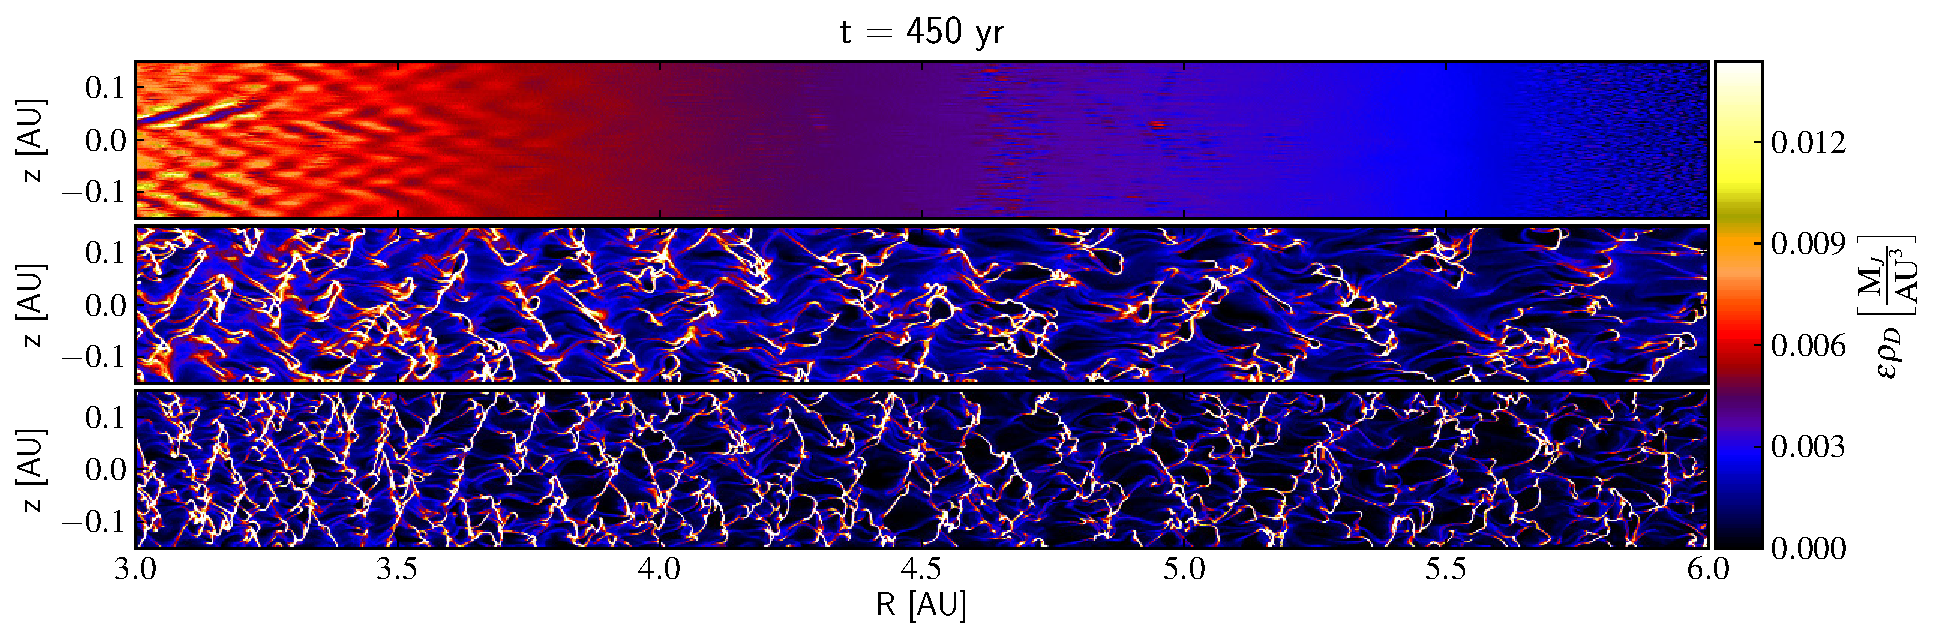
\includegraphics[width=0.49\linewidth]{figures/fig1c} &
      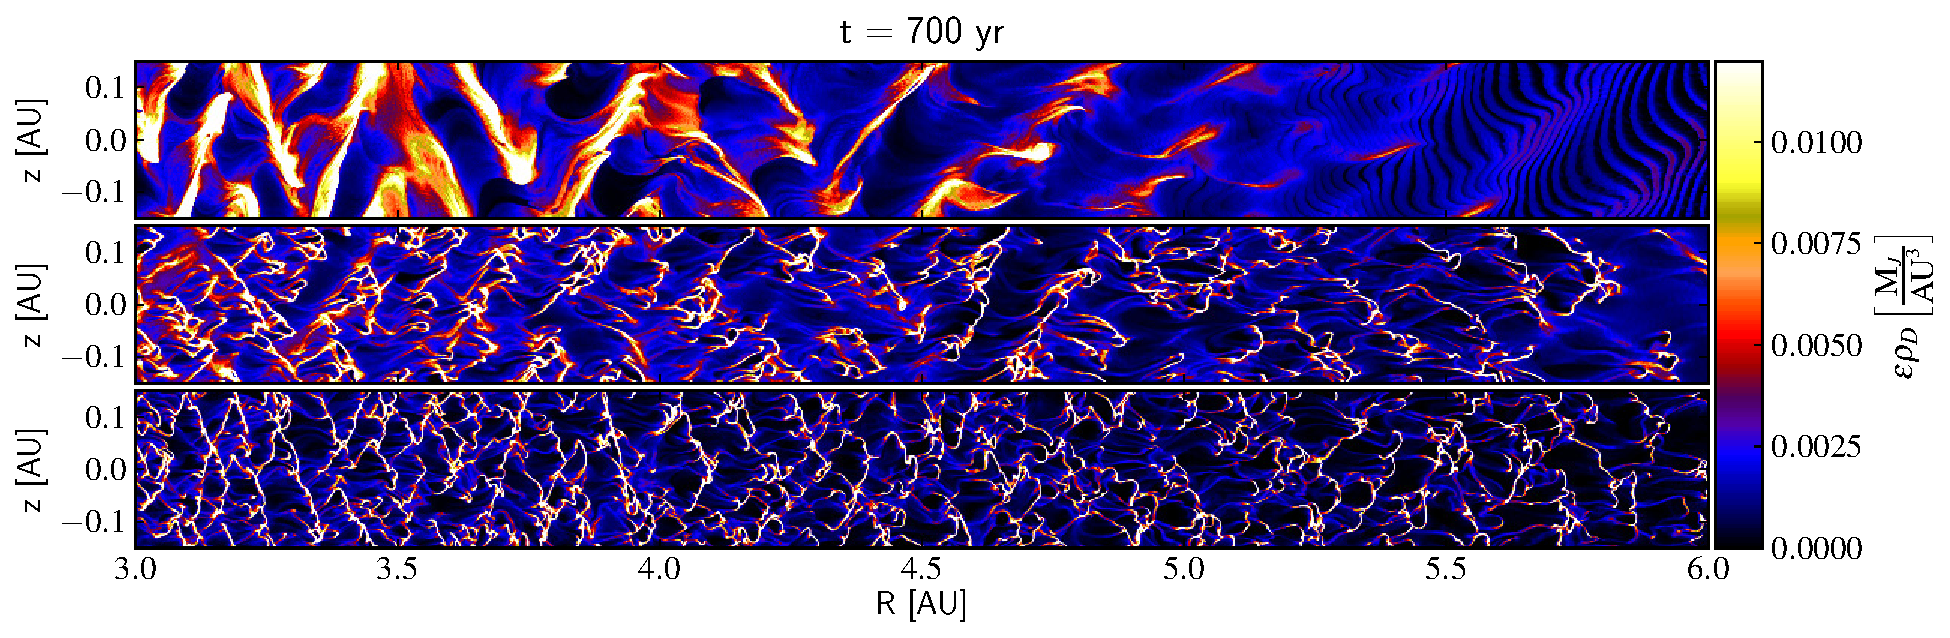
\includegraphics[width=0.49\linewidth]{figures/fig1d}
   \end{tabular}
   \caption{Migawki gęstości pyłu dla symulacji z $50$~cm ziarnami pyłu
      dla czasu $100$, $200$, $450$ oraz $700$~lat odpowiednio dla lewego
      górnego, prawego górnego, dolnego lewego i dolnego prawego panelu.
      Każdy z paneli jest podzielony na trzy części różniące się początkowym 
      $\epsilon = 0.2, 1, 2.0$ odpowiednio dla górnego (BAh), środkowego (BB) i
      dolnego (BC) podpanelu.}
   \label{fig1}
\end{figure*}
%
\subsection{Liniowa analiza stabilności}
\label{sec:lsa}
Jednym z celów naukowych poniższej pracy jest walidacja wyników eksperymentu
numerycznego poprzez porównanie z tempem wzrostu najsilniejszych modów
otrzymanych z liniowej analizy stabilności. W tym rozdziale przedstawiono
poszczególne kroki liniowej analizy stabilności dla niestabilności strumieniowej
w oparciu o pracę~\citep{YG05}.

Analiza stabilności opiera się na trzech elementach:
\begin{enumerate}
   \item znalezieniu stanu równowagi dla zadanego układu równań,
   \item zaburzeniu układu znaną funkcją o małej amplitudzie 
   \item wyprowadzeniu modów własnych oraz ich tempa wzrostu.
\end{enumerate}
Niestety dla układu równań hydrodynamiki dwóch sprzężonych płynów w rozciągłym
dysku keplerowskim nie istnieje warunek równowagowy. Spowodowane jest to
migracja pyłu na centrum grawitacji na skutek utraty momemtu pędu przez tarcie
aerodynamiczne. Naturalną konsekwencją migracji są znaczne zmiany w radialnym
profilu rozkładu gęstości pyłu. Należy jednak zauważyć, że charakterystyczna
skala czasowa migracji jest rzędu setek bądź wiecej lat, przy założeniu iż mamy
do czynienia z aglomeratami pyłu o rozmiarach metrowych. Z tego względu możemy
założyć że zmiany w profilu gęstości są procesem powolnym w stosunku do typowego
tempa wzrostu niestabilności strumieniowej, co zostanie wykazane w dalszej
części wywodu.

Kolejną przeszkodą jest sama rozciągłość symulowanego dysku okołogwiazdowego,
która implikuje zmienność potencjalnego stanu równowagowego wraz z promieniem
dysku. W tym wypadku powinno przeprowadzić się globalną analizę stabilności po
przez rozwiązanie dwupunktowego problem brzegowego (np.~\cite{PHM04, KH06}),
jednakże takie podejście jest dużo bardziej skomplikowane. Przedstawianą tu
lokalną analizę należy zatem traktować jako pierwsze przybliżenie pełnej analizy
stabilności niestabiności strumieniowej. Niestabilne mody uzyskane w ramach
liniowej analizy posłużą nam jako punkt odniesienia dla modów uzyskiwanych w
globalnym eksperymencie numerycznym.

Najbardziej wygodnym układem do lokalnego opisu niestabilności strumieniowej
jest tzw. kostka ścinana~\footnote{ang. shearing box}~\citep{HGB95}, czyli
kartezjański układ współrzędnych, którego początek współporusza się z płynem na
wybranej orbicie $R_0$ z częstością keplerowską $\Omega_0 \equiv
\Omega\left(R_0\right)$. Zwyczajowo przyjmuje się, że oś $x$ jest skierowana
radialnie na zewnątrz, oś $y$ jest w kierunku azymutalnym, zaś $z$ jest osią
wertykalną. Zgodnie z pracą~\cite*{YJ07} układ równań ciągłości oraz ruchu dla
obu składników można wyrazić poprzez:
%
\begin{align}
\partial_t \rho_g &+ \mathbf{u}\cdot\nabla\rho_g - \frac{3}{2}\Omega x\partial_y\rho_g 
 = -\rho_g\nabla\cdot\mathbf{u},\label{eqc1}\\
\partial_t \rho_d &+ \mathbf{w}\cdot\nabla\rho_d - \frac{3}{2}\Omega x\partial_y\rho_d 
 = -\rho_d\nabla\cdot\mathbf{w},\label{eqc2}\\
\partial_t \mathbf{u} &+ \left(\mathbf{u}\cdot\nabla\right)\mathbf{u} 
 - \frac{3}{2}\Omega x\partial_y\mathbf{u} 
 = 2\Omega u_y \hat{\mathbf{x}} -\frac{1}{2}\Omega u_x \hat{\mathbf{y}} \notag\\
 &- \frac{\epsilon}{\tau_f}(\mathbf{u}-\mathbf{w}) -c_s^2\nabla\ln\rho_g 
 +2\eta\Omega^2 R \hat{\mathbf{x}},\label{eqm1}\\
\partial_t \mathbf{w} &+ \left(\mathbf{w}\cdot\nabla\right)\mathbf{w} 
 - \frac{3}{2}\Omega x\partial_y\mathbf{w}
 = 2\Omega w_y \hat{\mathbf{x}} -\frac{1}{2}\Omega w_x \hat{\mathbf{y}} \notag\\
 &- \frac{1}{\tau_f}(\mathbf{w}-\mathbf{u}), \label{eqm2}
\end{align}
%
gdzie wyrazy takie jak $(3/2)\Omega x$ po lewej stronie równań, pojawiają się na
skutek relatywizacji wszytkich predkości względem liniowego, ścinanego przepływu
$\mathbf{v}_0 = -(3/2)\Omega x \hat{\mathbf{y}}$ w rotującym układzie
współrzędnych. Warto nadmienić, że wyraz $-(1/2)\Omega \{u,w\}_x
\hat{\mathbf{y}}$ po prawej stronie równań ruchu \mref{eqm1}-\mref{eqm2} jest
sumą dwóch składników: $(-2\Omega \{u,w\}_x + (3/2)\Omega \{u,w\}_x)
\hat{\mathbf{y}}$ z których pierwszy jest składową siły Coriolisa, a drugi
wynika z odjęcia wspomnianego wcześniej przepływu średniego. Główną różnicą
pomiędzy równaniami \mref{eqm1} oraz \mref{eqm2} jest brak wyrazu ciśnieniowego
dla składnika pyłowego. Jak zauważyli YG05, można w spójny sposób uwzględnić
globalny, radialny gradient ciśnienia gazu ograniczając się do liniowego wyrazu,
który jest zparametryzowany tzw. bezwymiarową miarą rotacji podkeplerowskiej:

\begin{equation}
\eta \equiv - \frac{\partial_R P}{2\rho_g\Omega^2 R} \sim \frac{c_s^2}{v_K^2}.
\end{equation}

Układ równań \mref{eqc1}-\mref{eqm2} posiada znane rozwiązanie równowagowe~\citep{N86}

\begin{align}
\bar{\mathbf{w}} &= \left[ 
 -2\tau_s\xi, \frac{\tau_s^2\xi - 1}{1+\epsilon},
 0
\right]\eta v_K, \label{eq:w0}\\
\bar{\mathbf{u}} &= \left[ 
 2\epsilon\tau_s\xi, -\frac{1 + \epsilon\tau_s^2\xi}{1+\epsilon},
 0
\right]\eta v_K, \label{eq:u0}
\end{align}
%
gdzie $\tau_s = \Omega \tau_f$ to dimensionless stopping time i 
$\xi = ((1+\epsilon)^2 + \tau_s^2)^{-1}$. 
Linearyzacja równań \mref{eqc1}-\mref{eqm2}, polega na rozbiciu zmiennych na
część stałą oraz zaburzenie $\mathbf{q} = \bar{\mathbf{q}} + \mathbf{q}^\prime$,
gdzie $\mathbf{q}=[\rho_d, w_x, w_y, w_z, \rho_g, u_x, u_y, u_z]$. Zakładamy
równocześnie, że zaburzenie jest osiowosymetryczne (niezależne od współrzędnej $y$)
i przyjmuje postać fali płaskiej:

\begin{equation}
   \label{eq:planar}
   \mathbf{q}^\prime(x,z,t) = \tilde{\mathbf{q}}
 \exp\left[i(k_x x + k_z z -\omega t)\right]
\end{equation}

Po podstawieniu liniowego zaburzenia układ równań przyjmuje następującą postać

\begin{align}
-i(\omega- k_x\bar{w}_x)\tilde{\rho}_d &= 
 - i \bar{\rho}_d(k_x\tilde{w}_x + k_z\tilde{w}_z), \label{lin1}\\
-i(\omega- k_x\bar{u}_x)\tilde{\rho}_g &= 
 - i \bar{\rho}_g(k_x\tilde{u}_x + k_z\tilde{u}_z), \label{lin2}\\
-i(\omega- k_x\bar{u}_x)\tilde{\mathbf{u}} &= 
 2\Omega \tilde{u}_y\hat{\mathbf{x}} - \frac{1}{2}\Omega \tilde{u}_x
 \hat{\mathbf{y}}
 -\frac{\epsilon}{\tau_f}(\tilde{\mathbf{u}} - \tilde{\mathbf{w}}) \notag\\
  -\frac{\tilde{\rho}_d}{\bar{\rho}_g\tau_f}
  (\bar{\mathbf{u}} &- \bar{\mathbf{w}})
  - \frac{c_s^2}{\bar{\rho}_g}ik_x\tilde{\rho}_g\hat{\mathbf{x}} -
  - \frac{c_s^2}{\bar{\rho}_g}ik_z\tilde{\rho}_g\hat{\mathbf{z}}, \label{lin3}\\
-i(\omega- k_x\bar{w}_x)\tilde{\mathbf{w}} &= 
 2\Omega \tilde{w}_y\hat{\mathbf{x}} - \frac{1}{2}\Omega \tilde{w}_x
 \hat{\mathbf{y}} 
 - \frac{1}{\tau_f} (\tilde{\mathbf{w}} - \tilde{\mathbf{u}}), \label{lin4}
\end{align}
%
gdzie $\epsilon = \bar{\rho}_d/\bar{\rho}_g$. Układ równań
\mref{lin1}-\mref{lin4} można zapisać jako

\begin{equation}
 \eurom{A}(k_x,k_z,\omega)\tilde{\mathbf{q}} = 0
 \label{eq:linset}
\end{equation}
%
Nietrywialne rozwiązania układu linoweg \mref{eq:linset} istnieją wtedy i tylko
wtedy gdy równanie dyspersyjne 
\begin{equation}
 \det|\eurom{A}(k_x,k_z,\omega)|=0.
 \label{eq:disprel}
\end{equation}
%
Dla zadanych wartości $(k_x, k_x)$ relację \mref{eq:disprel} można rozwiąć ze
względu na $\omega$ i dzięki temu otrzymać związki pomiędzy amplitudami
składowych wektora $\tilde{\mathbf{q}}$.
We solve the dispersion relation \mref{eq:disprel} for given values of
$(k_x,k_z)$, with respect to the complex frequency $\omega$, using the
Tempo wzrostu niestabilności definiujemy jako urojoną część zespolonej
częstotliwości $s=\Im(\omega)$.
%
\begin{figure*}
   \centering
   \begin{tabular}{@{}cc@{}}
      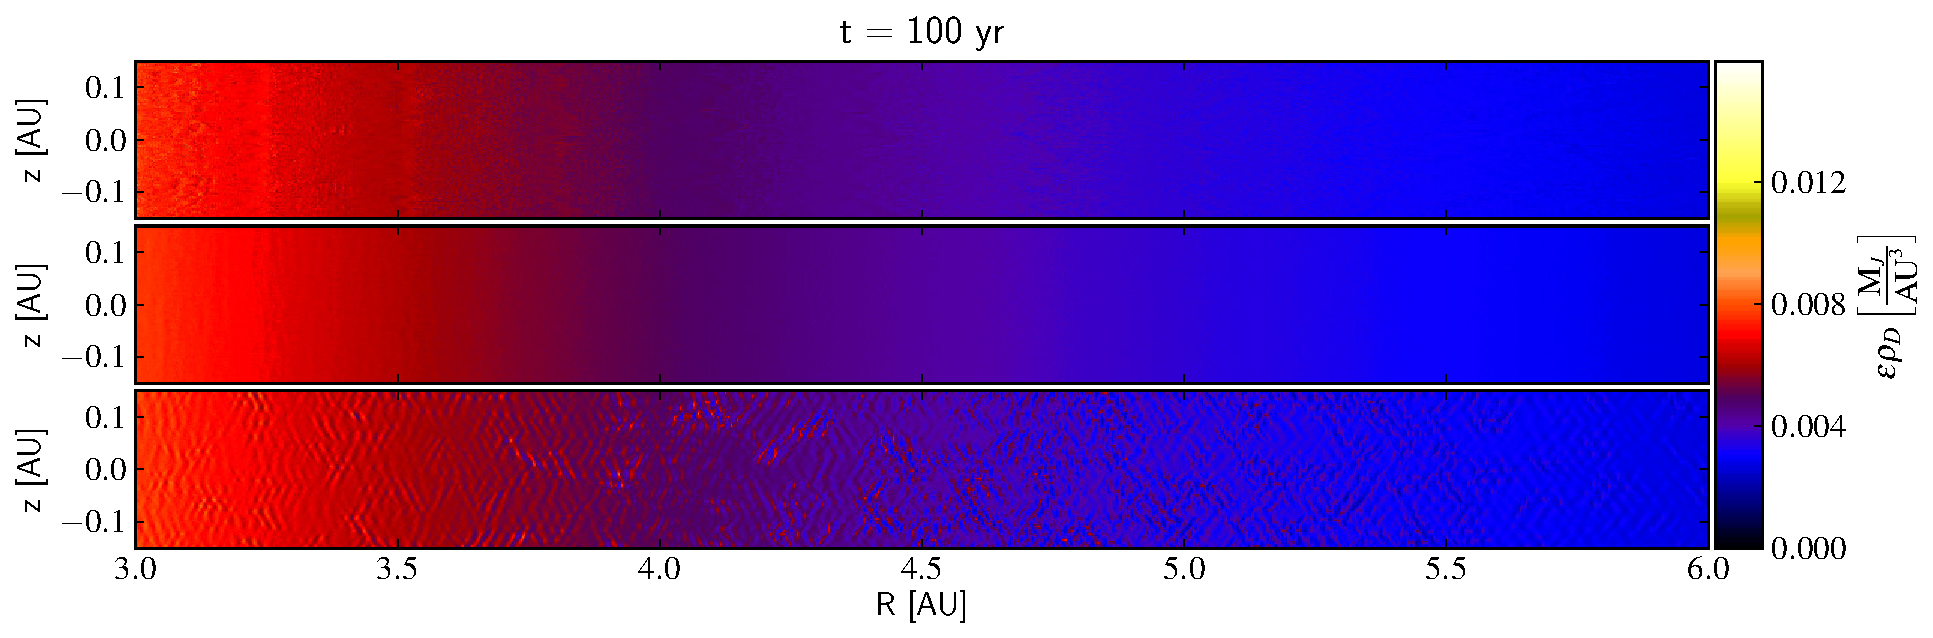
\includegraphics[width=0.49\linewidth]{figures/fig2a} &
      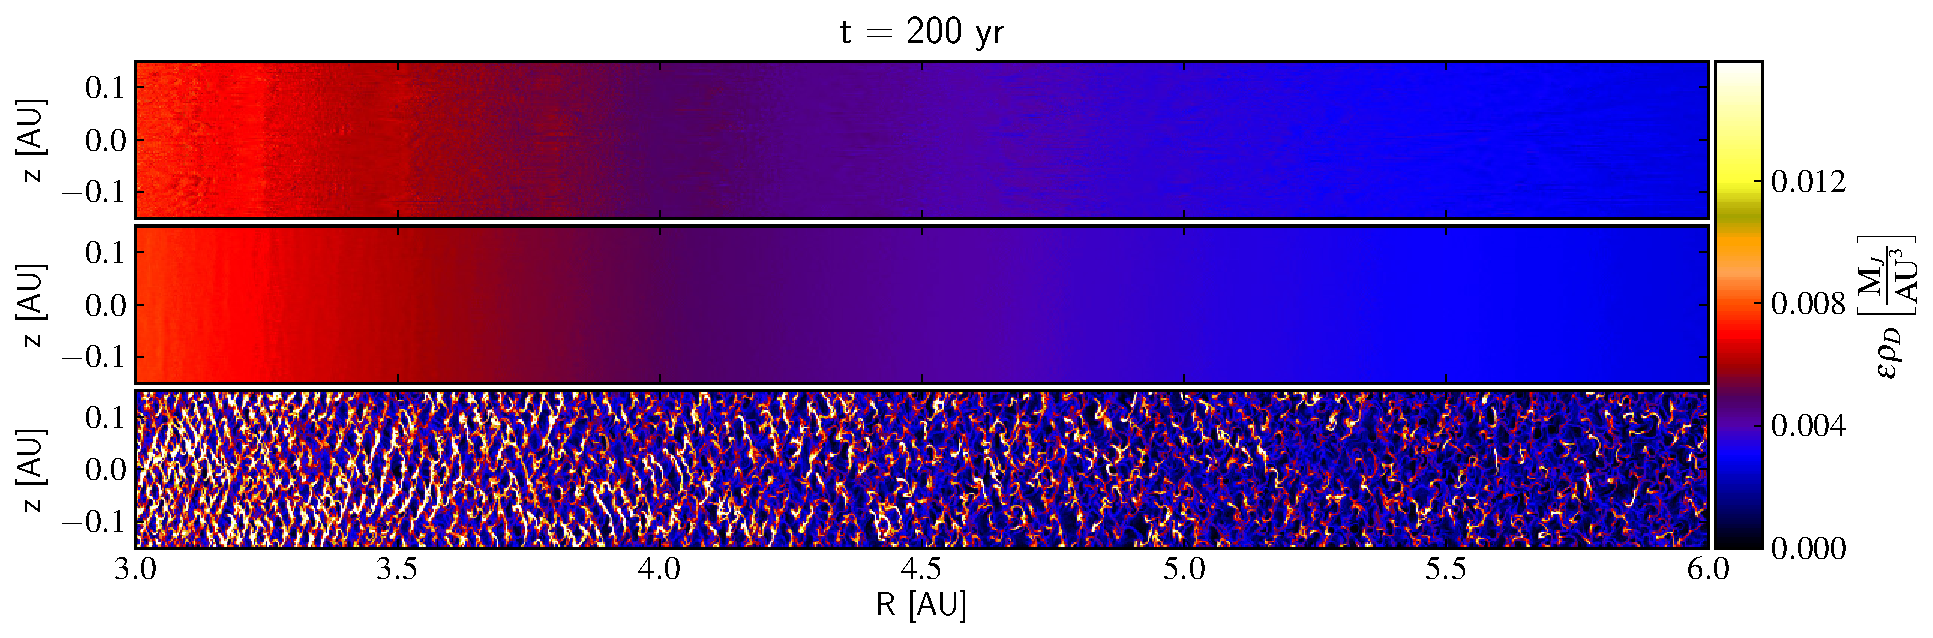
\includegraphics[width=0.49\linewidth]{figures/fig2b} \\
      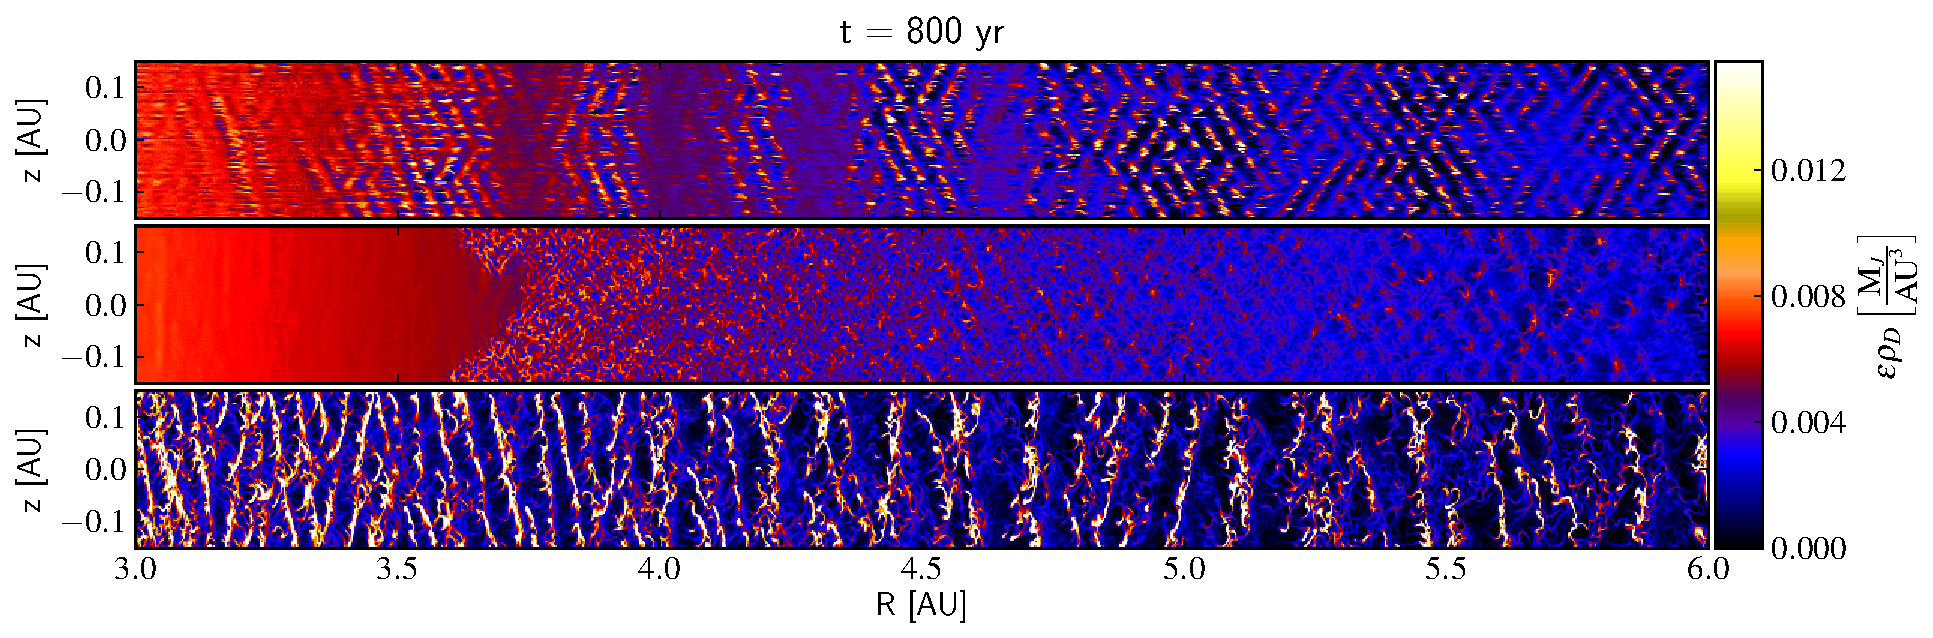
\includegraphics[width=0.49\linewidth]{figures/fig2c} &
      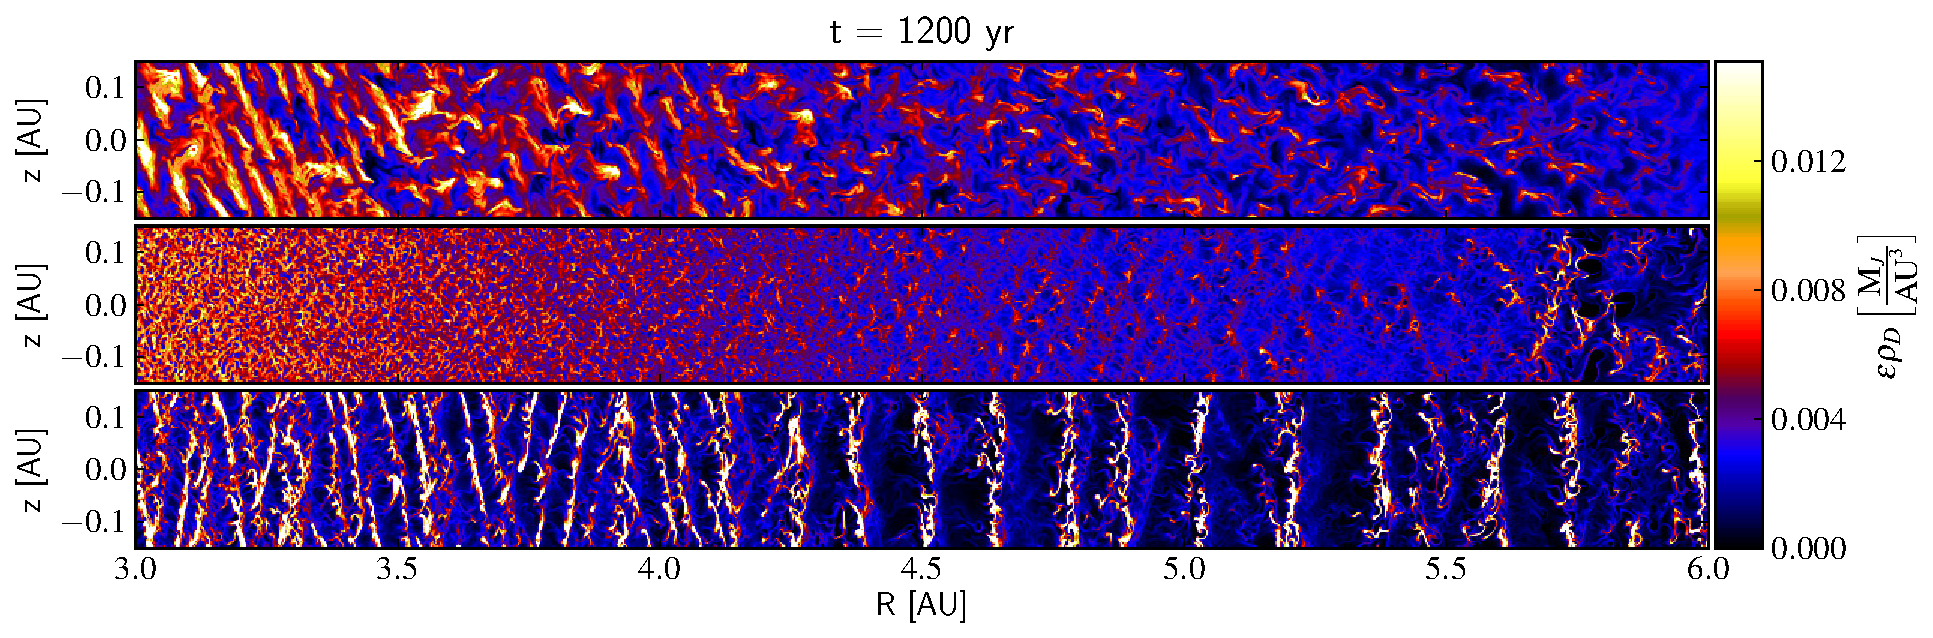
\includegraphics[width=0.49\linewidth]{figures/fig2d}
   \end{tabular}
   \caption{Migawki gęstości pyłu dla symulacji z $10$~cm ziarnami pyłu
      dla czasu $100$, $200$, $800$ oraz $1200$~lat odpowiednio dla lewego
      górnego, prawego górnego, dolnego lewego i dolnego prawego panelu.
      Każdy z paneli jest podzielony na trzy części różniące się początkowym 
      $\epsilon = 0.2, 1, 2.0$ odpowiednio dla górnego (AA), środkowego (AB) i
      dolnego (AC) podpanelu.}
   \label{fig2}
\end{figure*}
\subsection{FARGO}

\subsection{Schemat implicit dla oddziaływania}
Both components i.e. gas and dust are treated as fluids~\citep{piernik2} which
are dynamically coupled via the friction force. In order to prevent large
timestep constraint from drag force acceleration we used the semi-implicit
scheme by~\cite{TB09}. We allow the system to relax numerically (during the
period of initial $10$~yrs of the simulation) before we ''turn on'' the
aerodynamic drag force and seed dust velocities with low--amplitude random
noise. The feedback of the linear drag force scales with the density ratio of
dust to gas $\epsilon\equiv \rho_d/\rho_g$.

\subsection{Potencjał grawitacyjny}
\section{Warunki początkowe}
The initial density profile for gas roughly follows prescription of Minimal Mass
Solar Nebula~\citep{H81}
\begin{equation}
   \Sigma(R) = 1700 \left(\frac{R}{1\textrm{ AU}}\right)^{-3/2} 
   \textrm{ g cm}^{-2}.
\end{equation}
We assume isothermal equation of state and a constant temperature $T_0 = 170$~K
across the whole disc. 
We assume gravitational field from a point mass $M=1\,\textrm{M}_\odot$, and
neglect the vertical component of gravitational acceleration towards the central
mass, implying no vertical stratification of the disc. Yet, we refer to the
vertical scaleheight $H$ to estimate  volume density of gas at given radius,
relying on the hydrostatic equilibrium density distribution in the presence of
the vertical gravity of a point mass
%
\begin{equation}
   \rho(R,z) =  \rho(R,0) \exp\left(-\frac{z^2}{2H(R)^2}\right),
\end{equation}
where $\rho(R,0)$ is gas density at the disc midplane and $H^2 = 2 c_s^2 R^3/
GM$.
%
The surface gas density is given by
\begin{equation}
   \Sigma(R) = \int_{-\infty}^\infty \rho(R,z) dz,
\end{equation}
%
The corresponding value of midplane gas density is
\begin{equation}
   \label{eq:rho}
    \rho(R,0) = \frac{\Sigma(R) }{\int_{-\infty}^\infty
   \exp\left(-\frac{z^2}{2H(R)^2}\right) dz}.
\end{equation}
For the chosen disc temperature $T_0$ the integral on the right hand side of
\mref{eq:rho} varies from $0.4$~AU to $2.0$~AU over the range of radii $R\in
[2,6]$~AU. 
We assume for simplicity its value equal to $1$~AU. 

We assume the vertical extent of the computational domain $L_z = 0.3$~AU, and
impose periodic boundary conditions at upper and lower $z$-boundaries. The
initial condition relies on a radial force balance for the gas and dust
components independently. The gas component remains in a hydrostatic equilibrium
resulting from the radial balance of gravity, centrifugal and pressure forces,
while the pressure gradient term is absent in the equation of motion for the
dust component.  Reflecting boundary conditions are set on the inner and outer
boundaries of the computational grid to prevent mass escape from the
computational domain. 

\par To minimise unphysical wave reflections, we implement wave killing zones
close to the inner and outer radial boundaries. The inner wave killing zones
cover 0.5 AU near the inner and outer edges of the computational domain. In
these zones, we add an additional damping term, in the evolution equations of
each fluid variable

\begin{equation}
  \frac{\textrm{d}X}{\textrm{d}t} = - \frac{X-X_0}{T_d}f(R),
\end{equation}
together with
\begin{equation}
   \begin{split} 
      f(R) &= 1 - \tanh\left(\left(R - R_\textrm{in} + 1
      \right)^{f_\textrm{in}}\right)\\ &+ \max\left\{ \tanh\left(\left(R -
      R_\textrm{out} + 1\right)^{f_\textrm{out}}\right), 0\right\}, 
   \end{split}
\end{equation}
where $X_0$ is the initial value of $X$ and $T_d$ is the damping timescale. We
chose $T_d$ of the order of orbital period.  The exponents
$f_\textrm{in}=f_\textrm{out}=10$ control the width of the transition layer
between the unmodified to the damped zones. Within the damped zones, the effects
of undesired wave reflection are essentially minimised.
%
\subsection{Simulation parameters}
%
We have performed a parameter sweep for the ratio of dust to gas density
$\epsilon$ and the size of particles $a$, at two different resolutions of the
computational grid in 2D, and additionally we have realized one of the models in
3D. Our choice of these parameters follows closely that of JY07, to enable
detailed comparison of the results.

The full list of simulations together with their main parameters is presented in
Table~\ref{tab1}. In all simulations the domain has height of $0.293$~AU,
for 2D it covers radii from 2 to 7~AU, whereas BB3D extends from 2 to 12~AU and
spans $\varphi\in[0, \pi/6]$.  Following JY07 we vary $\epsilon$ from 0.2 to
2.0~in order to exhibit morphologically different outcomes of nonlinear phase of
streaming instability.  We choose particle radii to be grater than $10$~cm and
less than $50$~cm so that (1) particles fall into Epstein regime in all
simulations, (2) their size could be plausibly explained by the growth processes
e.g. collisional agglomeration.

\begin{table}
   \centering
   \begin{tabular}{cccccc}
      \hline
      Run & $N_r \times N_\varphi \times N_z$ &
      $a$~[cm] & $\epsilon$ & $T_\textrm{end}$~[yr] \\
      \hline
      BB3D &  $5120  \times 128 \times 150$  & 50  & 1.0 & 500  \\
      AA   &  $5120  \times 1   \times 300$  & 10  & 0.2 & 3000 \\
      AB   &  $5120  \times 1   \times 300$  & 10  & 1.0 & 3000 \\
      AC   &  $5120  \times 1   \times 300$  & 10  & 2.0 & 3000 \\
      BA   &  $5120  \times 1   \times 300$  & 50  & 0.2 & 3000 \\
      BB   &  $5120  \times 1   \times 300$  & 50  & 1.0 & 3000 \\
      BC   &  $5120  \times 1   \times 300$  & 50  & 2.0 & 3000 \\
      AAh  &  $10240 \times 1   \times 600$  & 10  & 0.2 & 1700 \\
      AAu  &  $20480 \times 1   \times 1200$ & 10  & 0.2 & 1800 \\
      ABh  &  $10240 \times 1   \times 600$  & 10  & 1.0 & 1400 \\
      BAh  &  $10240 \times 1   \times 600$  & 50  & 0.2 & 1730 \\
      BBh  &  $10240 \times 1   \times 600$  & 50  & 1.0 & 3000 \\
      \hline
   \end{tabular}
\caption{Simulation parameters. Columns give, from left to right, name of the
   run, span of the computational domain in AU (r,z) and azimuthal angle, grid
   resolution, particle diameter in cm, solids-to-gas ratio, and total run time
   in units of years.} 
\label{tab1} 
\end{table}
